\chapter{Algoritmos de cadenas}

Este capítulo trata de algoritmos eficientes para el procesamiento
de cadenas o \textit{strings}. Muchos problemas en cadenas pueden
resolverse fácilmente en $O(n^2)$, pero el desafío está en encontrar
algoritmos que funcionen en $O(n)$ u $O(n \log n)$.

\index{búsqueda de patrones}

Por ejemplo, un problema fundamental en el procesamiento de cadenas
es la \key{búsqueda de patrones}: dada una cadena de longitud $n$ y
un patrón de longitud $m$, nuestra tarea es encontrar las ocurrencias
del patrón en la cadena. Por ejemplo, el patrón \texttt{ABC} ocurre
dos veces en la cadena \texttt{ABABCBABC}.

El problema de búsqueda de patrones puede resolverse fácilmente en
$O(nm)$ mediante un algoritmo de fuerza bruta que revisa todas las
posiciones en las cuales el patrón puede ocurrir en la cadena.
Sin embargo, en este capítulo veremos que existen algoritmos más
eficientes que solo requieren tiempo $O(n+m)$.

\index{cadena}
\indexalt{string}

\section{Terminología de cadenas}

\index{alfabeto}

A lo largo de este capítulo usaremos indexación basada
en cero en nuestras cadenas. Por ende, una cadena \texttt{s} de tamaño
$n$ consiste de los caracteres
$\texttt{s}[0],\ldots,\texttt{s}[n-1]$.
El conjunto de caracteres que forman a las cadenas se denomina
\key{alfabeto}. Por ejemplo, el alfabeto
$\{\texttt{A},\texttt{B},\ldots,\texttt{Z}\}$
consiste de las letras mayúsculas del español.

\index{subcadena}

Una \key{subcadena} es una secuencia de caracteres consecutivos dentro
de una cadena. Utilizamos la notación $\texttt{s}[a \ldots b]$ para
referirnos a la subcadena de \texttt{s} que comienza en la posición
$a$ y termina en la posición $b$. Una cadena de longitud $n$ tiene
$n(n+1)/2$ subcadenas. Por ejemplo, las subcadenas de \texttt{ABCD} son
\texttt{A}, \texttt{B}, \texttt{C}, \texttt{D},
\texttt{AB}, \texttt{BC}, \texttt{CD},
\texttt{ABC}, \texttt{BCD}, y \texttt{ABCD}.

\index{subsecuencia}

Una \key{subsecuencia} es una secuencia de caracteres, no necesariamente
consecutivos, de una cadena en su orden original. Una cadena de
longitud $n$ tiene $2^n-1$ subsecuencias. Por ejemplo, las subsecuencias
de \texttt{ABCD} son
\texttt{A}, \texttt{B}, \texttt{C}, \texttt{D},
\texttt{AB}, \texttt{AC}, \texttt{AD},
\texttt{BC}, \texttt{BD}, \texttt{CD},
\texttt{ABC}, \texttt{ABD}, \texttt{ACD},
\texttt{BCD}, y \texttt{ABCD}.

\index{prefijo}
\index{sufijo}

Un \key{prefijo} es una subcadena que comienza al inicio de una cadena,
y un \key{sufijo} es una cadena que termina al final de una cadena. Por
ejemplo, los prefijos de \texttt{ABCD} son
\texttt{A}, \texttt{AB}, \texttt{ABC}, y \texttt{ABCD},
y los sufijos de \texttt{ABCD} son
\texttt{D}, \texttt{CD}, \texttt{BCD}, y \texttt{ABCD}.

\index{rotación}

Una \key{rotación} puede generarse moviendo los caracteres de una
cadena uno tras otro de izquierda a derecha (o vice versa).
Por ejemplo, las rotaciones de \texttt{ABCD} son
\texttt{ABCD}, \texttt{BCDA}, \texttt{CDAB}, y \texttt{DABC}.

\index{periodo}

Un \key{periodo} es un prefijo de una cadena tal que la cadena puede
representarse repitiendo el periodo. La última repetición puede ser
parcial y solo contener un prefijo del periodo. Por ejemplo, el
mínimo periodo de \texttt{ABCABCA} es \texttt{ABC}.

\index{borde}

Un \key{borde} es una cadena que es tanto prefijo como sufijo de una
cadena. Por ejemplo, los bordes de \texttt{ABACABA} son \texttt{A},
\texttt{ABA}, y \texttt{ABACABA}.

\index{ordenamiento!lexicográfico}

Las cadenas se comparan utilizando el \key{orden lexicográfico},
que corresponde al orden alfabético. Significa que $x<y$ si $x \neq y$ y
$x$ es prefijo de $y$, \emph{o} si existe una posición $k$ tal que
$x[i]=y[i]$ donde $i<k$ y $x[k]<y[k]$.

\section{Estructura trie}

\index{trie}

Un \key{trie}\footnote{Pronunciado \textit{trai} o \textit{tri}, el nombre
    viene del inglés \textit{retrieval} ``recuperación'' (de información).}
es un árbol con raíz que guarda un conjunto de cadenas. Cada cadena se
almacena como un enlace de caracteres que comienza en la raíz. Si dos
cadenas tienen un prefijo en común también tienen un enlace en común
dentro del árbol.

Por ejemplo, considera el siguiente trie:

\begin{center}
    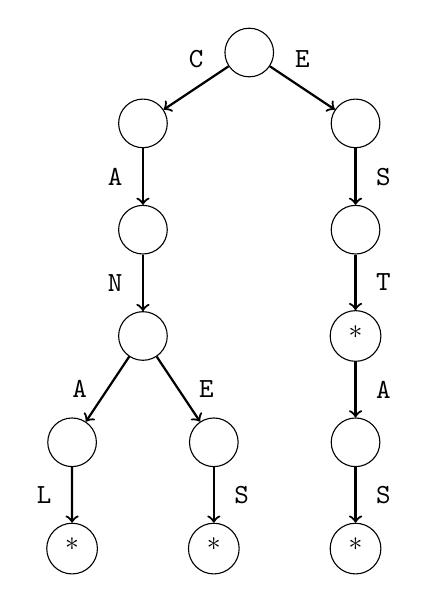
\begin{tikzpicture}[scale=0.9]
        \node[draw, circle] (1) at (0,20) {$\phantom{1}$};
        \node[draw, circle] (2) at (-1.5,19) {$\phantom{1}$};
        \node[draw, circle] (3) at (1.5,19) {$\phantom{1}$};
        \node[draw, circle] (4) at (-1.5,17.5) {$\phantom{1}$};
        \node[draw, circle] (5) at (-1.5,16) {$\phantom{1}$};
        \node[draw, circle] (6) at (-2.5,14.5) {$\phantom{1}$};
        \node[draw, circle] (7) at (-0.5,14.5) {$\phantom{1}$};
        \node[draw, circle] (8) at (-2.5,13) {*};
        \node[draw, circle] (9) at (-0.5,13) {*};
        \node[draw, circle] (10) at (1.5,17.5) {$\phantom{1}$};
        \node[draw, circle] (11) at (1.5,16) {*};
        \node[draw, circle] (12) at (1.5,14.5) {$\phantom{1}$};
        \node[draw, circle] (13) at (1.5,13) {*};

        \path[draw,thick,->] (1) -- node[font=\small,label=\texttt{C}] {} (2);
        \path[draw,thick,->] (1) -- node[font=\small,label=\texttt{E}] {} (3);
        \path[draw,thick,->] (2) -- node[font=\small,label=left:\texttt{A}] {} (4);
        \path[draw,thick,->] (4) -- node[font=\small,label=left:\texttt{N}] {} (5);
        \path[draw,thick,->] (5) -- node[font=\small,label=left:\texttt{A}] {} (6);
        \path[draw,thick,->] (5) -- node[font=\small,label=right:\texttt{E}] {} (7);
        \path[draw,thick,->] (6) -- node[font=\small,label=left:\texttt{L}] {}(8);
        \path[draw,thick,->] (7) -- node[font=\small,label=right:\texttt{S}] {} (9);
        \path[draw,thick,->] (3) -- node[font=\small,label=right:\texttt{S}] {} (10);
        \path[draw,thick,->] (10) -- node[font=\small,label=right:\texttt{T}] {} (11);
        \path[draw,thick,->] (11) -- node[font=\small,label=right:\texttt{A}] {} (12);
        \path[draw,thick,->] (12) -- node[font=\small,label=right:\texttt{S}] {} (13);
    \end{tikzpicture}
\end{center}

Este trie corresponde al conjunto
$\{\texttt{CANAL},\texttt{CANES},\texttt{ES},\texttt{ESTAS}\}$.
El carácter * en un nodo quiere decir que una cadena del conjunto
determina en ese nodo. Este carácter es necesario, porque una cadena
puede ser prefijo de otra cadena. Por ejemplo, en el trie de arriba,
\texttt{ES} es un prefijo de \texttt{ESTAS}.

Podemos revisar en tiempo $O(n)$ si un trie contiene una cadena de
longitud $n$, porque podemos seguir el enlace que comienza en el nodo raíz.
También podemos añadir una cadena de longitud $n$ al trie en tiempo $O(n)$
si seguimos la cadena y añadimos nodos cuando sea necesario.

Usando un trie, podemos encontrar el prefijo más largo de una cadena dada
tal que el prefijo pertenezca al conjunto. Además, si almacenamos
información adicional en cada nodo, podemos calcular el número de cadenas
que pertenecen al conjunto y poseen una cadena como prefijo.

\pagebreak \noindent
Podemos almacenar un trie en un arreglo
\begin{lstlisting}
int trie[N][A];
\end{lstlisting}
donde $N$ es el número máximo de nodos (la longitud máxima total
de las cadenas en el conjunto) y $A$ es el tamaño del alfabeto.
Los nodos de un trie se numeran $0,1,2,\ldots$ tal que el número de la
raíz es 0, y $\texttt{trie}[s][c]$ es el siguiente nodo en la cadena
cuando nos movemos del nodo $s$ usando el carácter $c$.

\section{\textit{Hashing} de cadenas}

\index{hashing}

El \key{\textit{hashing} de cadenas} es una técnica que nos permite
eficientemente revisar si dos cadenas son iguales.\footnote{La técnica se
    popularizó por el algoritmo de búsqueda de patrones de
    Rabin--Karp \cite{kar87}.}
La idea es comparar valores de hash en vez de los caracteres individuales.

\subsubsection*{Calcular hashes}

El \key{valor de hash} de una cadena es el número calculado en base a
los caracteres de la misma. Si dos cadenas son iguales, sus valores de
hash también son iguales, lo que nos permite comparar cadenas en base
a sus valores de hash.

Una manera típica de implementar el hashing de cadenas es usando
\key{hashing polinómico}, que significa que el valor de hash de una cadena
\texttt{s} de longitud $n$ es
\[(\texttt{s}[0] A^{n-1} + \texttt{s}[1] A^{n-2} + \cdots + \texttt{s}[n-1] A^0) \bmod B  ,\]
donde $s[0],s[1],\ldots,s[n-1]$ son interpretados como los códigos de
los caracteres de \texttt{s}, y $A$ y $B$ son constantes predefinidas.

Por ejemplo, los códigos de los caracteres de \texttt{SILLA} son:
\begin{center}
    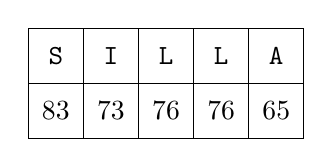
\begin{tikzpicture}[scale=0.7]
        \draw (0,0) grid (5,2);

        \node at (0.5, 1.5) {\texttt{S}};
        \node at (1.5, 1.5) {\texttt{I}};
        \node at (2.5, 1.5) {\texttt{L}};
        \node at (3.5, 1.5) {\texttt{L}};
        \node at (4.5, 1.5) {\texttt{A}};

        \node at (0.5, 0.5) {83};
        \node at (1.5, 0.5) {73};
        \node at (2.5, 0.5) {76};
        \node at (3.5, 0.5) {76};
        \node at (4.5, 0.5) {65};

    \end{tikzpicture}
\end{center}

Por ende, si $A=3$ y $B=97$, el valor de hash de \texttt{SILLA} es
\[(83 \cdot 3^4 + 73 \cdot 3^3 + 76 \cdot 3^2 + 76 \cdot 3^1 + 65 \cdot 3^0) \bmod 97 = 68.\]

\subsubsection*{Preprocesamiento}

Utilizando hashing polinómico, podemos calcular el valor de hash de
cualquier subcadena de una cadena \texttt{s} en tiempo $O(1)$ luego de un
preprocesamiento en $O(n)$. La idea es construir un arreglo \texttt{h} tal
que $\texttt{h}[k]$ contenga el valor de hash del prefijo
$\texttt{s}[0 \ldots k]$. Los valores del arreglo pueden calcularse de la
siguiente manera:
\[
    \begin{array}{lcl}
        \texttt{h}[0] & = & \texttt{s}[0]                               \\
        \texttt{h}[k] & = & (\texttt{h}[k-1] A + \texttt{s}[k]) \bmod B \\
    \end{array}
\]
Adicionalmente, construimos un arreglo $\texttt{p}$ donde
$\texttt{p}[k]=A^k \bmod B$:
\[
    \begin{array}{lcl}
        \texttt{p}[0] & = & 1                            \\
        \texttt{p}[k] & = & (\texttt{p}[k-1] A) \bmod B. \\
    \end{array}
\]
Construir estos arreglos tarda $O(n)$. Luego de esto, el valor de hash
de cualquier subcadena $\texttt{s}[a \ldots b]$ puede calcularse en
$O(1)$ usando la fórmula
\[(\texttt{h}[b]-\texttt{h}[a-1] \texttt{p}[b-a+1]) \bmod B\]
asumiendo que $a>0$. Si $a=0$, el valor de hash es simplemente
$\texttt{h}[b]$.

\subsubsection*{Usar valores de hash}

Podemos comparar cadenas eficientemente usando hashing. En vez
de comparar los caracteres individuales de las cadenas, la idea es comparar
sus valores de hash. Si los valores de hash son iguales, las cadenas
\emph{probablemente} son iguales, y si los valores son diferentes, las
cadenas \emph{ciertamente} son diferentes.

A menudo, el hashing nos permite optimizar algoritmos de fuerza bruta.
Por ejemplo, considera el problema de búsqueda de patrones: dada una cadena
$s$ y un patrón $p$, encuentra las posiciones donde $p$ ocurre en $s$.
Un algoritmo de fuerza bruta recorre todas las posiciones donde $p$
podría ocurrir y compara las cadenas carácter por carácter. La complejidad
temporal de un algoritmo tal es $O(n^2)$.

Podemos optimizar el algoritmo de fuerza bruta utilizando hashing,
porque el algoritmo compara subcadenas de las cadenas dadas.
Con hashing, cada comparación tarda solamente $O(1)$, porque solo
los valores de hash de las subcadenas se comparan. Esto resulta en un
algoritmo con complejidad temporal $O(n)$, que es la mejor complejidad
temporal posible para este problema.

Si combinamos el hashing y la \emph{búsqueda binaria}, también es posible
encontrar el orden lexicográfico de dos cadenas en tiempo logarítmico.
Podemos hacer esto si calculamos la longitud del prefijo común de las
cadenas usando búsqueda binaria. Una vez que sabemos la longitud del
prefijo común, podemos simplemente revisar el siguiente carácter luego
del prefijo, porque este determina el orden de las cadenas.

\subsubsection*{Parámetros y colisiones}

\index{colisión}

Un riesgo evidente cuando comparamos valores de hash es la \key{colisión},
que significa que dos cadenas sean diferentes pero sus valores de hash
sean iguales. En este caso, un algoritmo que depende en los valores de hash
concluye que las cadenas son iguales cuando realmente no lo son, y por lo
tanto puede devolver resultados incorrectos.

Las colisiones siempre son posibles, porque el número de cadenas diferentes
es mayor que el número de valores de hash diferentes. Sin embargo, la
probabilidad de una colisión es pequeña si las constantes $A$ y $B$ se
eligen con cuidado. Una manera común es elegir constantes aleatorias cerca
de $10^9$, por ejemplo así:
\[
    \begin{array}{lcl}
        A & = & 911382323 \\
        B & = & 972663749 \\
    \end{array}
\]

Utilizando tales constantes, el tipo \texttt{long long} puede utilizarse
cuando calculamos valores de hash, porque los productos $AB$ y $BB$
entrarán en \texttt{long long}. Pero, ¿es suficiente tener alrededor
de $10^9$ valores de hash distintos?

Consideremos tres situaciones donde podemos utilizar hashing:

\textit{Situación 1}: Las cadenas $x$ e $y$ se comparan una con otra.
La probabilidad de una colisión es $1/B$ asumiendo que todos los valores
de hash son igual de probables.

\textit{Situación 2}: Una cadena $x$ se compara con cadenas
$y_1,y_2,\ldots,y_n$. La probabilidad de una o más colisiones es de

\[1-\left(1-\frac{1}{B}\right)^n.\]

\textit{Situación 3}: Todos los pares de cadenas $x_1,x_2,\ldots,x_n$
se comparan entre ellas. La probabilidad de una o más colisiones es de
\[ 1 - \frac{B \cdot (B-1) \cdot (B-2) \cdots (B-n+1)}{B^n}.\]

La siguiente tabla muestra las probabilidades de colisión cuando
$n=10^6$ y el valor de $B$ varía:

\begin{center}
    \begin{tabular}{rrrr}
        constante $B$ & situación 1 & situación 2 & situación 3 \\
        \hline
        $10^3$        & $0,001000$  & $1,000000$  & $1,000000$  \\
        $10^6$        & $0,000001$  & $0,632121$  & $1,000000$  \\
        $10^9$        & $0,000000$  & $0,001000$  & $1,000000$  \\
        $10^{12}$     & $0,000000$  & $0,000000$  & $0,393469$  \\
        $10^{15}$     & $0,000000$  & $0,000000$  & $0,000500$  \\
        $10^{18}$     & $0,000000$  & $0,000000$  & $0,000001$  \\
    \end{tabular}
\end{center}

La tabla muestra que en la situación 1, la probabilidad de una colisión
es despreciable cuando $B \approx 10^9$. En la situación 2, una colisión
es posible pero la probabilidad es aún bastante pequeña. No obstante, en
la situación 3 cambian las cosas: una colisión casi siempre sucede cuando
$B \approx 10^9$.

\index{paradoja del cumpleaños}

El fenómeno en la situación 3 se conoce como la \key{paradoja del
    cumpleaños}: si hay $n$ personas en una habitación, la probabilidad de
que \emph{algún} par de personas compartan cumpleaños es grande incluso
si $n$ es bastante pequeña. En el hashing corresponde que cuando todos
los valores de hash se comparan el uno con otro, la probabilidad de que
dos valores sean iguales es grande.

Podemos disminuir la probabilidad de colisión si calculamos \emph{múltiples}
valores de hash utilizando diferentes parámetros. Es improbable que una
colisión ocurra en todos los valores de hash al mismo tiempo. Por ejemplo,
dos valores de hash con el parámetro $B \approx 10^9$ corresponden a un
valor de hash con el parámetro $B \approx 10^{18}$, lo que hace la
probabilidad de colisión muy pequeña.

Algunas personas utilizan las constantes $B=2^{32}$ y $B=2^{64}$, que
es conveniente, porque las operaciones con enteros de 32 y 64 bits
son calculadas módulo $2^{32}$ y $2^{64}$. Sin embargo, esta \emph{no}
es una buena decisión, porque es posible construir entradas que siempre
generan colisiones cuando se utilizan constantes con la forma
$2^x$ \cite{pac13}.

\section{Algoritmo Z}

\index{algoritmo!Z}
\index{arreglo Z}

El \key{arreglo Z}, denominado \texttt{z}, de una cadena \texttt{s} con
longitud $n$ contiene para cada $k=0,1,\ldots,n-1$ la longitud de la
subcadena más larga de \texttt{s} que comienza en la posición $k$ y es
a la vez un prefijo de \texttt{s}. Por ende, $\texttt{z}[k]=p$ nos dice que
$\texttt{s}[0 \ldots p-1]$ equivale a $\texttt{s}[k \ldots k+p-1]$.
Muchos problemas de procesamiento de cadenas pueden resolverse
eficientemente utilizando el arreglo Z.

Por ejemplo, el arreglo Z de la cadena
\texttt{ACBACDACBACBACDA} es el siguiente:

\begin{center}
    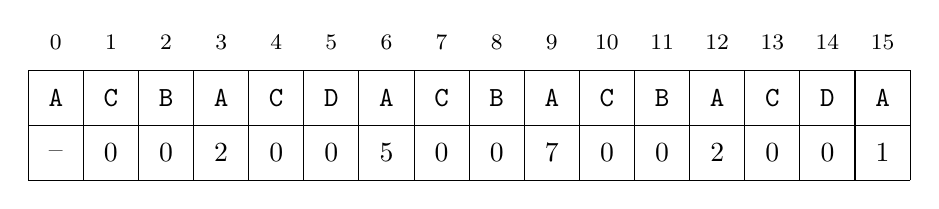
\begin{tikzpicture}[scale=0.7]
        \draw (0,0) grid (16,2);

        \node at (0.5, 1.5) {\texttt{A}};
        \node at (1.5, 1.5) {\texttt{C}};
        \node at (2.5, 1.5) {\texttt{B}};
        \node at (3.5, 1.5) {\texttt{A}};
        \node at (4.5, 1.5) {\texttt{C}};
        \node at (5.5, 1.5) {\texttt{D}};
        \node at (6.5, 1.5) {\texttt{A}};
        \node at (7.5, 1.5) {\texttt{C}};
        \node at (8.5, 1.5) {\texttt{B}};
        \node at (9.5, 1.5) {\texttt{A}};
        \node at (10.5, 1.5) {\texttt{C}};
        \node at (11.5, 1.5) {\texttt{B}};
        \node at (12.5, 1.5) {\texttt{A}};
        \node at (13.5, 1.5) {\texttt{C}};
        \node at (14.5, 1.5) {\texttt{D}};
        \node at (15.5, 1.5) {\texttt{A}};

        \node at (0.5, 0.5) {--};
        \node at (1.5, 0.5) {0};
        \node at (2.5, 0.5) {0};
        \node at (3.5, 0.5) {2};
        \node at (4.5, 0.5) {0};
        \node at (5.5, 0.5) {0};
        \node at (6.5, 0.5) {5};
        \node at (7.5, 0.5) {0};
        \node at (8.5, 0.5) {0};
        \node at (9.5, 0.5) {7};
        \node at (10.5, 0.5) {0};
        \node at (11.5, 0.5) {0};
        \node at (12.5, 0.5) {2};
        \node at (13.5, 0.5) {0};
        \node at (14.5, 0.5) {0};
        \node at (15.5, 0.5) {1};

        \footnotesize
        \node at (0.5, 2.5) {0};
        \node at (1.5, 2.5) {1};
        \node at (2.5, 2.5) {2};
        \node at (3.5, 2.5) {3};
        \node at (4.5, 2.5) {4};
        \node at (5.5, 2.5) {5};
        \node at (6.5, 2.5) {6};
        \node at (7.5, 2.5) {7};
        \node at (8.5, 2.5) {8};
        \node at (9.5, 2.5) {9};
        \node at (10.5, 2.5) {10};
        \node at (11.5, 2.5) {11};
        \node at (12.5, 2.5) {12};
        \node at (13.5, 2.5) {13};
        \node at (14.5, 2.5) {14};
        \node at (15.5, 2.5) {15};

    \end{tikzpicture}
\end{center}

En este caso, por ejemplo, $\texttt{z}[6]=5$, porque la subcadena
\texttt{ACBAC} de longitud 5 es un prefijo de \texttt{s}, pero la
subcadena \texttt{ACBACB} de longitud 6 no es un prefijo de \texttt{s}.

\subsubsection*{Descripción del algoritmo}

Ahora describiremos un algoritmo, llamado el \key{algoritmo Z},\footnote{
    El algoritmo Z fue presentado en \cite{gus97} como el método más
    simple conocido para la búsqueda de patrones en tiempo lineal, y la
    idea original es atribuida a \cite{mai84}.
} que construye el arreglo Z eficientemente en tiempo $O(n)$. Este
algoritmo calcula los valores del arreglo Z de izquierda a derecha
tanto utilizando información ya almacenada en el arreglo como
comparando subcadenas carácter por carácter.

Para calcular los valores del arreglo Z eficientemente, el algoritmo
mantiene un rango $[x,y]$ tal que $\texttt{s}[x \ldots y]$ sea un
prefijo de \texttt{s} e $y$ sea tan grande como sea posible. Ya que
sabemos que $\texttt{s}[0 \ldots y-x]$ y $\texttt{s}[x \ldots y]$ son
iguales, podemos usar esta información al calcular valores del arreglo
Z para las posiciones $x+1,x+2,\ldots,y$.

En cada posición $k$, primero revisamos el valor de $\texttt{z}[k-x]$.
Si $k+\texttt{z}[k-x]<y$, sabemos que $\texttt{z}[k]=\texttt{z}[k-x]$.
Sin embargo, si $k+\texttt{z}[k-x] \ge y$, $\texttt{s}[0 \ldots y-k]$
es igual a $\texttt{s}[k \ldots y]$ y para determinar $\texttt{z}[k]$
necesitamos comparar las subcadenas carácter por carácter. No obstante,
el algoritmo funciona en tiempo $O(n)$, porque comenzamos comparando en
las posiciones $y-k+1$ y $y+1$.

Por ejemplo, vamos a construir el siguiente arreglo Z:

\begin{center}
    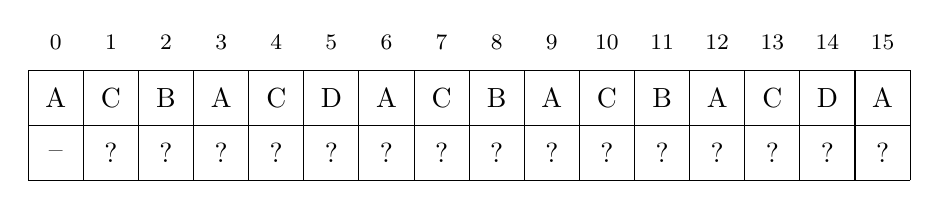
\begin{tikzpicture}[scale=0.7]
        \draw (0,0) grid (16,2);

        \node at (0.5, 1.5) {A};
        \node at (1.5, 1.5) {C};
        \node at (2.5, 1.5) {B};
        \node at (3.5, 1.5) {A};
        \node at (4.5, 1.5) {C};
        \node at (5.5, 1.5) {D};
        \node at (6.5, 1.5) {A};
        \node at (7.5, 1.5) {C};
        \node at (8.5, 1.5) {B};
        \node at (9.5, 1.5) {A};
        \node at (10.5, 1.5) {C};
        \node at (11.5, 1.5) {B};
        \node at (12.5, 1.5) {A};
        \node at (13.5, 1.5) {C};
        \node at (14.5, 1.5) {D};
        \node at (15.5, 1.5) {A};

        \node at (0.5, 0.5) {--};
        \node at (1.5, 0.5) {?};
        \node at (2.5, 0.5) {?};
        \node at (3.5, 0.5) {?};
        \node at (4.5, 0.5) {?};
        \node at (5.5, 0.5) {?};
        \node at (6.5, 0.5) {?};
        \node at (7.5, 0.5) {?};
        \node at (8.5, 0.5) {?};
        \node at (9.5, 0.5) {?};
        \node at (10.5, 0.5) {?};
        \node at (11.5, 0.5) {?};
        \node at (12.5, 0.5) {?};
        \node at (13.5, 0.5) {?};
        \node at (14.5, 0.5) {?};
        \node at (15.5, 0.5) {?};

        \footnotesize
        \node at (0.5, 2.5) {0};
        \node at (1.5, 2.5) {1};
        \node at (2.5, 2.5) {2};
        \node at (3.5, 2.5) {3};
        \node at (4.5, 2.5) {4};
        \node at (5.5, 2.5) {5};
        \node at (6.5, 2.5) {6};
        \node at (7.5, 2.5) {7};
        \node at (8.5, 2.5) {8};
        \node at (9.5, 2.5) {9};
        \node at (10.5, 2.5) {10};
        \node at (11.5, 2.5) {11};
        \node at (12.5, 2.5) {12};
        \node at (13.5, 2.5) {13};
        \node at (14.5, 2.5) {14};
        \node at (15.5, 2.5) {15};

    \end{tikzpicture}
\end{center}

Luego de calcular el valor $\texttt{z}[6]=5$, el rango actual $[x,y]$
es $[6,10]$:

\begin{center}
    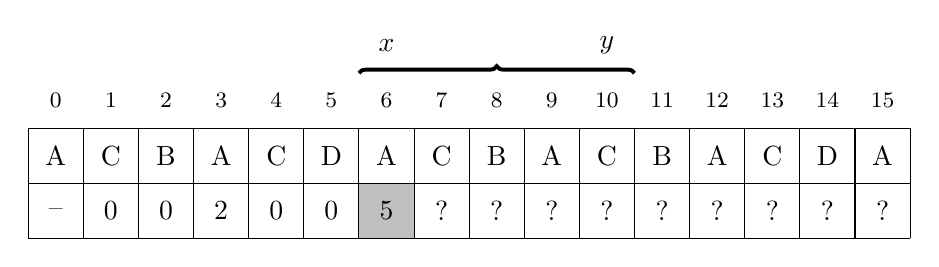
\begin{tikzpicture}[scale=0.7]
        \fill[color=lightgray] (6,0) rectangle (7,1);
        \draw (0,0) grid (16,2);

        \node at (0.5, 1.5) {A};
        \node at (1.5, 1.5) {C};
        \node at (2.5, 1.5) {B};
        \node at (3.5, 1.5) {A};
        \node at (4.5, 1.5) {C};
        \node at (5.5, 1.5) {D};
        \node at (6.5, 1.5) {A};
        \node at (7.5, 1.5) {C};
        \node at (8.5, 1.5) {B};
        \node at (9.5, 1.5) {A};
        \node at (10.5, 1.5) {C};
        \node at (11.5, 1.5) {B};
        \node at (12.5, 1.5) {A};
        \node at (13.5, 1.5) {C};
        \node at (14.5, 1.5) {D};
        \node at (15.5, 1.5) {A};

        \node at (0.5, 0.5) {--};
        \node at (1.5, 0.5) {0};
        \node at (2.5, 0.5) {0};
        \node at (3.5, 0.5) {2};
        \node at (4.5, 0.5) {0};
        \node at (5.5, 0.5) {0};
        \node at (6.5, 0.5) {5};
        \node at (7.5, 0.5) {?};
        \node at (8.5, 0.5) {?};
        \node at (9.5, 0.5) {?};
        \node at (10.5, 0.5) {?};
        \node at (11.5, 0.5) {?};
        \node at (12.5, 0.5) {?};
        \node at (13.5, 0.5) {?};
        \node at (14.5, 0.5) {?};
        \node at (15.5, 0.5) {?};

        \draw [decoration={brace}, decorate, line width=0.5mm] (6,3.00) -- (11,3.00);

        \node at (6.5,3.50) {$x$};
        \node at (10.5,3.50) {$y$};


        \footnotesize
        \node at (0.5, 2.5) {0};
        \node at (1.5, 2.5) {1};
        \node at (2.5, 2.5) {2};
        \node at (3.5, 2.5) {3};
        \node at (4.5, 2.5) {4};
        \node at (5.5, 2.5) {5};
        \node at (6.5, 2.5) {6};
        \node at (7.5, 2.5) {7};
        \node at (8.5, 2.5) {8};
        \node at (9.5, 2.5) {9};
        \node at (10.5, 2.5) {10};
        \node at (11.5, 2.5) {11};
        \node at (12.5, 2.5) {12};
        \node at (13.5, 2.5) {13};
        \node at (14.5, 2.5) {14};
        \node at (15.5, 2.5) {15};

    \end{tikzpicture}
\end{center}

Ahora podemos calcular valores subsecuentes del arreglo Z eficientemente,
porque sabemos que $\texttt{s}[0 \ldots 4]$ y $\texttt{s}[6 \ldots 10]$
son iguales. Primero, debido a que $\texttt{z}[1] = \texttt{z}[2] = 0$,
inmediatamente sabemos que $\texttt{z}[7] = \texttt{z}[8] = 0$:

\begin{center}
    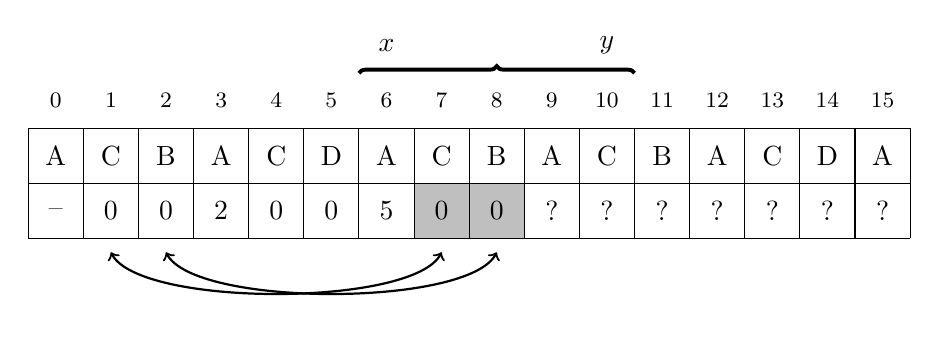
\begin{tikzpicture}[scale=0.7]
        \fill[color=lightgray] (7,0) rectangle (9,1);
        \draw (0,0) grid (16,2);

        \node at (0.5, 1.5) {A};
        \node at (1.5, 1.5) {C};
        \node at (2.5, 1.5) {B};
        \node at (3.5, 1.5) {A};
        \node at (4.5, 1.5) {C};
        \node at (5.5, 1.5) {D};
        \node at (6.5, 1.5) {A};
        \node at (7.5, 1.5) {C};
        \node at (8.5, 1.5) {B};
        \node at (9.5, 1.5) {A};
        \node at (10.5, 1.5) {C};
        \node at (11.5, 1.5) {B};
        \node at (12.5, 1.5) {A};
        \node at (13.5, 1.5) {C};
        \node at (14.5, 1.5) {D};
        \node at (15.5, 1.5) {A};

        \node at (0.5, 0.5) {--};
        \node at (1.5, 0.5) {0};
        \node at (2.5, 0.5) {0};
        \node at (3.5, 0.5) {2};
        \node at (4.5, 0.5) {0};
        \node at (5.5, 0.5) {0};
        \node at (6.5, 0.5) {5};
        \node at (7.5, 0.5) {0};
        \node at (8.5, 0.5) {0};
        \node at (9.5, 0.5) {?};
        \node at (10.5, 0.5) {?};
        \node at (11.5, 0.5) {?};
        \node at (12.5, 0.5) {?};
        \node at (13.5, 0.5) {?};
        \node at (14.5, 0.5) {?};
        \node at (15.5, 0.5) {?};


        \draw [decoration={brace}, decorate, line width=0.5mm] (6,3.00) -- (11,3.00);

        \node at (6.5,3.50) {$x$};
        \node at (10.5,3.50) {$y$};


        \footnotesize
        \node at (0.5, 2.5) {0};
        \node at (1.5, 2.5) {1};
        \node at (2.5, 2.5) {2};
        \node at (3.5, 2.5) {3};
        \node at (4.5, 2.5) {4};
        \node at (5.5, 2.5) {5};
        \node at (6.5, 2.5) {6};
        \node at (7.5, 2.5) {7};
        \node at (8.5, 2.5) {8};
        \node at (9.5, 2.5) {9};
        \node at (10.5, 2.5) {10};
        \node at (11.5, 2.5) {11};
        \node at (12.5, 2.5) {12};
        \node at (13.5, 2.5) {13};
        \node at (14.5, 2.5) {14};
        \node at (15.5, 2.5) {15};


        \draw[thick,<->] (7.5,-0.25) .. controls (7,-1.25) and (2,-1.25) .. (1.5,-0.25);
        \draw[thick,<->] (8.5,-0.25) .. controls (8,-1.25) and (3,-1.25) .. (2.5,-0.25);
    \end{tikzpicture}
\end{center}

Ahora, ya que $\texttt{z}[3]=2$, sabemos que $\texttt{z}[9] \ge 2$:

\begin{center}
    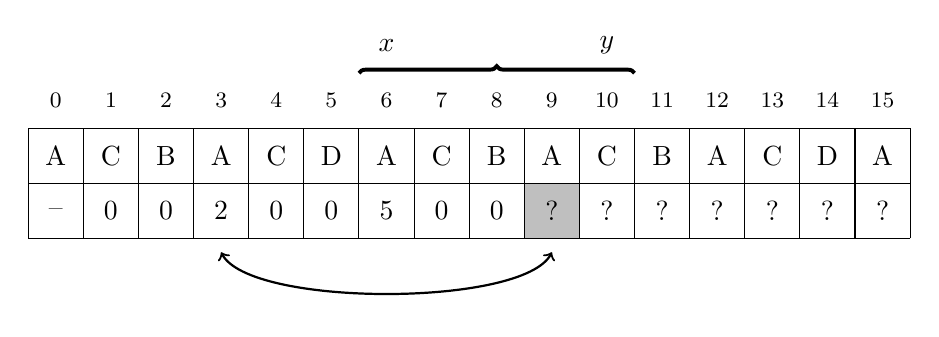
\begin{tikzpicture}[scale=0.7]
        \fill[color=lightgray] (9,0) rectangle (10,1);
        \draw (0,0) grid (16,2);

        \node at (0.5, 1.5) {A};
        \node at (1.5, 1.5) {C};
        \node at (2.5, 1.5) {B};
        \node at (3.5, 1.5) {A};
        \node at (4.5, 1.5) {C};
        \node at (5.5, 1.5) {D};
        \node at (6.5, 1.5) {A};
        \node at (7.5, 1.5) {C};
        \node at (8.5, 1.5) {B};
        \node at (9.5, 1.5) {A};
        \node at (10.5, 1.5) {C};
        \node at (11.5, 1.5) {B};
        \node at (12.5, 1.5) {A};
        \node at (13.5, 1.5) {C};
        \node at (14.5, 1.5) {D};
        \node at (15.5, 1.5) {A};

        \node at (0.5, 0.5) {--};
        \node at (1.5, 0.5) {0};
        \node at (2.5, 0.5) {0};
        \node at (3.5, 0.5) {2};
        \node at (4.5, 0.5) {0};
        \node at (5.5, 0.5) {0};
        \node at (6.5, 0.5) {5};
        \node at (7.5, 0.5) {0};
        \node at (8.5, 0.5) {0};
        \node at (9.5, 0.5) {?};
        \node at (10.5, 0.5) {?};
        \node at (11.5, 0.5) {?};
        \node at (12.5, 0.5) {?};
        \node at (13.5, 0.5) {?};
        \node at (14.5, 0.5) {?};
        \node at (15.5, 0.5) {?};

        \draw [decoration={brace}, decorate, line width=0.5mm] (6,3.00) -- (11,3.00);

        \node at (6.5,3.50) {$x$};
        \node at (10.5,3.50) {$y$};


        \footnotesize
        \node at (0.5, 2.5) {0};
        \node at (1.5, 2.5) {1};
        \node at (2.5, 2.5) {2};
        \node at (3.5, 2.5) {3};
        \node at (4.5, 2.5) {4};
        \node at (5.5, 2.5) {5};
        \node at (6.5, 2.5) {6};
        \node at (7.5, 2.5) {7};
        \node at (8.5, 2.5) {8};
        \node at (9.5, 2.5) {9};
        \node at (10.5, 2.5) {10};
        \node at (11.5, 2.5) {11};
        \node at (12.5, 2.5) {12};
        \node at (13.5, 2.5) {13};
        \node at (14.5, 2.5) {14};
        \node at (15.5, 2.5) {15};

        \draw[thick,<->] (9.5,-0.25) .. controls (9,-1.25) and (4,-1.25) .. (3.5,-0.25);
    \end{tikzpicture}
\end{center}

No obstante, no tenemos información sobre la cadena luego de la posición
10, por lo que debemos comparar las subcadenas carácter por carácter:

\begin{center}
    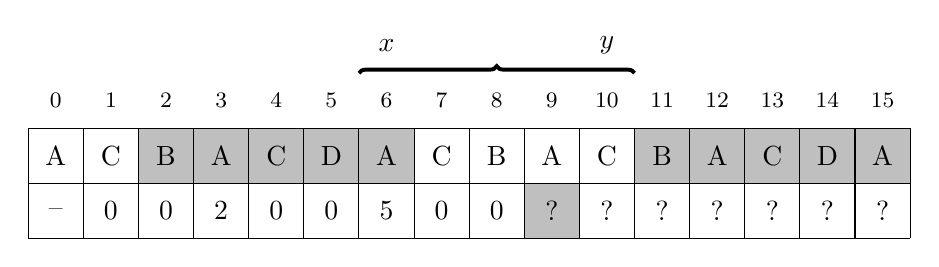
\begin{tikzpicture}[scale=0.7]
        \fill[color=lightgray] (9,0) rectangle (10,1);
        \fill[color=lightgray] (2,1) rectangle (7,2);
        \fill[color=lightgray] (11,1) rectangle (16,2);


        \draw (0,0) grid (16,2);

        \node at (0.5, 1.5) {A};
        \node at (1.5, 1.5) {C};
        \node at (2.5, 1.5) {B};
        \node at (3.5, 1.5) {A};
        \node at (4.5, 1.5) {C};
        \node at (5.5, 1.5) {D};
        \node at (6.5, 1.5) {A};
        \node at (7.5, 1.5) {C};
        \node at (8.5, 1.5) {B};
        \node at (9.5, 1.5) {A};
        \node at (10.5, 1.5) {C};
        \node at (11.5, 1.5) {B};
        \node at (12.5, 1.5) {A};
        \node at (13.5, 1.5) {C};
        \node at (14.5, 1.5) {D};
        \node at (15.5, 1.5) {A};

        \node at (0.5, 0.5) {--};
        \node at (1.5, 0.5) {0};
        \node at (2.5, 0.5) {0};
        \node at (3.5, 0.5) {2};
        \node at (4.5, 0.5) {0};
        \node at (5.5, 0.5) {0};
        \node at (6.5, 0.5) {5};
        \node at (7.5, 0.5) {0};
        \node at (8.5, 0.5) {0};
        \node at (9.5, 0.5) {?};
        \node at (10.5, 0.5) {?};
        \node at (11.5, 0.5) {?};
        \node at (12.5, 0.5) {?};
        \node at (13.5, 0.5) {?};
        \node at (14.5, 0.5) {?};
        \node at (15.5, 0.5) {?};

        \draw [decoration={brace}, decorate, line width=0.5mm] (6,3.00) -- (11,3.00);

        \node at (6.5,3.50) {$x$};
        \node at (10.5,3.50) {$y$};


        \footnotesize
        \node at (0.5, 2.5) {0};
        \node at (1.5, 2.5) {1};
        \node at (2.5, 2.5) {2};
        \node at (3.5, 2.5) {3};
        \node at (4.5, 2.5) {4};
        \node at (5.5, 2.5) {5};
        \node at (6.5, 2.5) {6};
        \node at (7.5, 2.5) {7};
        \node at (8.5, 2.5) {8};
        \node at (9.5, 2.5) {9};
        \node at (10.5, 2.5) {10};
        \node at (11.5, 2.5) {11};
        \node at (12.5, 2.5) {12};
        \node at (13.5, 2.5) {13};
        \node at (14.5, 2.5) {14};
        \node at (15.5, 2.5) {15};

        %\draw[thick,<->] (11.5,-0.25) .. controls (11,-1.25) and (3,-1.25) .. (2.5,-0.25);
    \end{tikzpicture}
\end{center}

Resulta que $\texttt{z}[9]=7$, así que el nuevo rango $[x,y]$ es $[9,15]$:

\begin{center}
    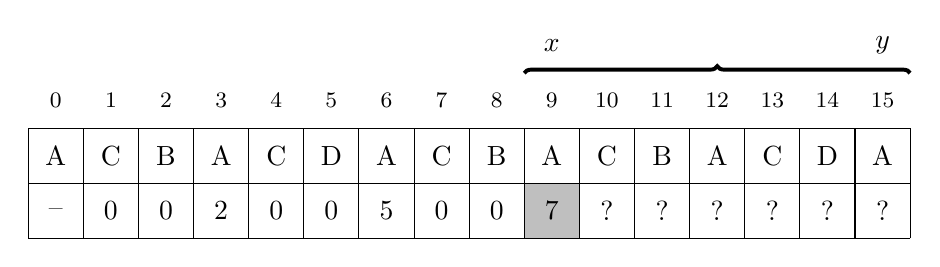
\begin{tikzpicture}[scale=0.7]
        \fill[color=lightgray] (9,0) rectangle (10,1);
        \draw (0,0) grid (16,2);

        \node at (0.5, 1.5) {A};
        \node at (1.5, 1.5) {C};
        \node at (2.5, 1.5) {B};
        \node at (3.5, 1.5) {A};
        \node at (4.5, 1.5) {C};
        \node at (5.5, 1.5) {D};
        \node at (6.5, 1.5) {A};
        \node at (7.5, 1.5) {C};
        \node at (8.5, 1.5) {B};
        \node at (9.5, 1.5) {A};
        \node at (10.5, 1.5) {C};
        \node at (11.5, 1.5) {B};
        \node at (12.5, 1.5) {A};
        \node at (13.5, 1.5) {C};
        \node at (14.5, 1.5) {D};
        \node at (15.5, 1.5) {A};

        \node at (0.5, 0.5) {--};
        \node at (1.5, 0.5) {0};
        \node at (2.5, 0.5) {0};
        \node at (3.5, 0.5) {2};
        \node at (4.5, 0.5) {0};
        \node at (5.5, 0.5) {0};
        \node at (6.5, 0.5) {5};
        \node at (7.5, 0.5) {0};
        \node at (8.5, 0.5) {0};
        \node at (9.5, 0.5) {7};
        \node at (10.5, 0.5) {?};
        \node at (11.5, 0.5) {?};
        \node at (12.5, 0.5) {?};
        \node at (13.5, 0.5) {?};
        \node at (14.5, 0.5) {?};
        \node at (15.5, 0.5) {?};

        \draw [decoration={brace}, decorate, line width=0.5mm] (9,3.00) -- (16,3.00);

        \node at (9.5,3.50) {$x$};
        \node at (15.5,3.50) {$y$};


        \footnotesize
        \node at (0.5, 2.5) {0};
        \node at (1.5, 2.5) {1};
        \node at (2.5, 2.5) {2};
        \node at (3.5, 2.5) {3};
        \node at (4.5, 2.5) {4};
        \node at (5.5, 2.5) {5};
        \node at (6.5, 2.5) {6};
        \node at (7.5, 2.5) {7};
        \node at (8.5, 2.5) {8};
        \node at (9.5, 2.5) {9};
        \node at (10.5, 2.5) {10};
        \node at (11.5, 2.5) {11};
        \node at (12.5, 2.5) {12};
        \node at (13.5, 2.5) {13};
        \node at (14.5, 2.5) {14};
        \node at (15.5, 2.5) {15};

        % \draw[thick,<->] (9.5,-0.25) .. controls (9,-1.25) and (4,-1.25) .. (3.5,-0.25);
    \end{tikzpicture}
\end{center}

Luego de esto, todos los valores restantes pueden determinarse
utilizando información que ya está almacenada en el arreglo Z:

\begin{center}
    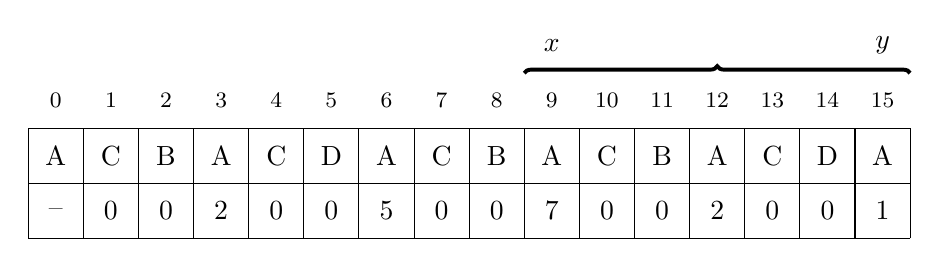
\begin{tikzpicture}[scale=0.7]
        \draw (0,0) grid (16,2);

        \node at (0.5, 1.5) {A};
        \node at (1.5, 1.5) {C};
        \node at (2.5, 1.5) {B};
        \node at (3.5, 1.5) {A};
        \node at (4.5, 1.5) {C};
        \node at (5.5, 1.5) {D};
        \node at (6.5, 1.5) {A};
        \node at (7.5, 1.5) {C};
        \node at (8.5, 1.5) {B};
        \node at (9.5, 1.5) {A};
        \node at (10.5, 1.5) {C};
        \node at (11.5, 1.5) {B};
        \node at (12.5, 1.5) {A};
        \node at (13.5, 1.5) {C};
        \node at (14.5, 1.5) {D};
        \node at (15.5, 1.5) {A};

        \node at (0.5, 0.5) {--};
        \node at (1.5, 0.5) {0};
        \node at (2.5, 0.5) {0};
        \node at (3.5, 0.5) {2};
        \node at (4.5, 0.5) {0};
        \node at (5.5, 0.5) {0};
        \node at (6.5, 0.5) {5};
        \node at (7.5, 0.5) {0};
        \node at (8.5, 0.5) {0};
        \node at (9.5, 0.5) {7};
        \node at (10.5, 0.5) {0};
        \node at (11.5, 0.5) {0};
        \node at (12.5, 0.5) {2};
        \node at (13.5, 0.5) {0};
        \node at (14.5, 0.5) {0};
        \node at (15.5, 0.5) {1};

        \draw [decoration={brace}, decorate, line width=0.5mm] (9,3.00) -- (16,3.00);

        \node at (9.5,3.50) {$x$};
        \node at (15.5,3.50) {$y$};


        \footnotesize
        \node at (0.5, 2.5) {0};
        \node at (1.5, 2.5) {1};
        \node at (2.5, 2.5) {2};
        \node at (3.5, 2.5) {3};
        \node at (4.5, 2.5) {4};
        \node at (5.5, 2.5) {5};
        \node at (6.5, 2.5) {6};
        \node at (7.5, 2.5) {7};
        \node at (8.5, 2.5) {8};
        \node at (9.5, 2.5) {9};
        \node at (10.5, 2.5) {10};
        \node at (11.5, 2.5) {11};
        \node at (12.5, 2.5) {12};
        \node at (13.5, 2.5) {13};
        \node at (14.5, 2.5) {14};
        \node at (15.5, 2.5) {15};

    \end{tikzpicture}
\end{center}

\subsubsection{Usar el arreglo Z}

A menudo es una cuestión de gustos si usar hashing o el algoritmo Z.
A diferencia del hashing, el algoritmo Z siempre funciona ya que no hay
un riesgo de colisiones. Por otro lado, el algoritmo Z es más difícil de
implementar y algunos problemas solo pueden resolverse con hashing.

Por ejemplo, considera de nuevo el problema de búsqueda de patrones,
donde nuestra tarea es encontrar las ocurrencias de un patrón $p$ en
una cadena $s$. Ya resolvimos este problema eficientemente usando el
hashing de cadenas, pero el algoritmo Z es otra manera de resolverlo.

Una idea frecuente en el procesamiento de cadenas es construir una
cadena que consiste de múltiples cadenas separadas por caracteres
especiales. En este problema, podemos construir una cadena
$p$\texttt{\#}$s$, donde $p$ y $s$ están separados por un carácter
especial \texttt{\#} que no ocurre en las cadenas. El arreglo Z de
$p$\texttt{\#}$s$ nos dice las posiciones en donde $p$ ocurre en $s$,
porque tales posiciones contienen la longitud de $p$.

Por ejemplo, si $s=\texttt{PERROBARRO}$ y $p=\texttt{RRO}$, el
arreglo Z es el siguiente:

\begin{center}
    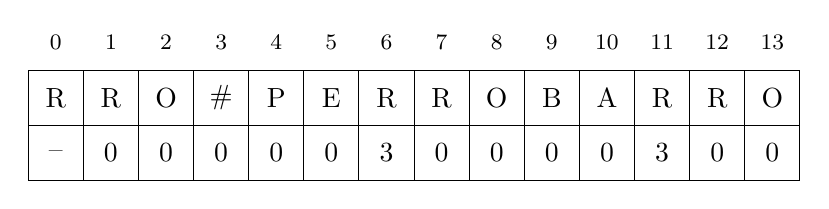
\begin{tikzpicture}[scale=0.7]
        \draw (0,0) grid (14,2);

        \node at (0.5, 1.5) {R};
        \node at (1.5, 1.5) {R};
        \node at (2.5, 1.5) {O};
        \node at (3.5, 1.5) {\#};
        \node at (4.5, 1.5) {P};
        \node at (5.5, 1.5) {E};
        \node at (6.5, 1.5) {R};
        \node at (7.5, 1.5) {R};
        \node at (8.5, 1.5) {O};
        \node at (9.5, 1.5) {B};
        \node at (10.5, 1.5) {A};
        \node at (11.5, 1.5) {R};
        \node at (12.5, 1.5) {R};
        \node at (13.5, 1.5) {O};

        \node at (0.5, 0.5) {--};
        \node at (1.5, 0.5) {0};
        \node at (2.5, 0.5) {0};
        \node at (3.5, 0.5) {0};
        \node at (4.5, 0.5) {0};
        \node at (5.5, 0.5) {0};
        \node at (6.5, 0.5) {3};
        \node at (7.5, 0.5) {0};
        \node at (8.5, 0.5) {0};
        \node at (9.5, 0.5) {0};
        \node at (10.5, 0.5) {0};
        \node at (11.5, 0.5) {3};
        \node at (12.5, 0.5) {0};
        \node at (13.5, 0.5) {0};

        \footnotesize
        \node at (0.5, 2.5) {0};
        \node at (1.5, 2.5) {1};
        \node at (2.5, 2.5) {2};
        \node at (3.5, 2.5) {3};
        \node at (4.5, 2.5) {4};
        \node at (5.5, 2.5) {5};
        \node at (6.5, 2.5) {6};
        \node at (7.5, 2.5) {7};
        \node at (8.5, 2.5) {8};
        \node at (9.5, 2.5) {9};
        \node at (10.5, 2.5) {10};
        \node at (11.5, 2.5) {11};
        \node at (12.5, 2.5) {12};
        \node at (13.5, 2.5) {13};
    \end{tikzpicture}
\end{center}

Las posiciones 6 y 11 contienen el valor 3, lo que significa que el
patrón \texttt{RRO} ocurre en las posiciones correspondientes de
\texttt{PERROBARRO}.

La complejidad temporal del algoritmo resultante es lineal, porque es
suficiente construir el arreglo Z y recorrer sus valores una vez.

\subsubsection{Implementación}

Aquí vemos una corta implementación del algoritmo Z que devuelve un
vector que corresponde al arreglo Z.

\begin{lstlisting}
vector<int> z(string s) {
    int n = s.size();
    vector<int> z(n);
    int x = 0, y = 0;
    for (int i = 1; i < n; i++) {
        z[i] = max(0, min(z[i - x], y - i + 1));
        while (i + z[i] < n && s[z[i]] == s[i + z[i]]) {
            x = i;
            y = i + z[i];
            z[i]++;
        }
    }
    return z;
}
\end{lstlisting}